\section{Поняття стійкості різницевих схем}

\shortLectureDescription{Поняття стійкості різницевих схем. Причини і види розповсюдження збурення. Поняття асимптотичної збіжності різницевих схем. Метод дискретних збурень. \cite{rouch1980, sam1983, richtmyer1972, kollatz}}

\subsection{Опис нестійкості}

Для ознайомлення з деякими феноменологічними аспектами чисельної нестійкості розглянемо одномірне модельне лінійне рівняння для $\zeta$. На мал.~\ref{fig:3.6}(а) показаний стаціонарний розв'язок $\hat{\zeta}^n$  на $n$-му часовому шарі, а на мал.~\ref{fig:3.6}(б) --- накладення на $\zeta^n$ збурення $\epsilon$, форма якого представлена на мал.~\ref{fig:3.6}(в). Такі збурення можуть породжуватися або машинними похибками округлення, або поперечними рухами у реальній двовимірній задачі. Використовуючи схему з різницями вперед за часом і центральними різницями по просторовій змінної, простежимо за розвитком накладеного збурення. Лінійне модельне рівняння в консервативній формі має вигляд
\begin{equation*}
    \frac{\partial \zeta}{\partial t} = - \frac{\partial (u \zeta)}{\partial x} + \alpha \frac{\partial^2 \zeta}{\partial x^2}
\end{equation*}
а різницеве --- вигляд
\begin{equation}
    \label{eq:3.48}
    \frac{\zeta_i^{n + 1} - \zeta_i^n}{\Delta t} = - \frac{u \zeta_{i + 1}^n - u \zeta_{i - 1}^n}{2 \Delta x} + \alpha \frac{\zeta_{i + 1}^n - 2 \zeta_i^n + \zeta_{i - 1}^n}{\Delta x^2}
\end{equation}
Представимо величину $\zeta$ як суму стаціонарної компоненти $\hat{\zeta}$ й збурення $\epsilon$:
\begin{equation}
    \label{eq:3.49}
    \zeta_i^n = \hat{\zeta}_i^n + \epsilon_i.
\end{equation}
 
\begin{figure}[H]
    \centering
    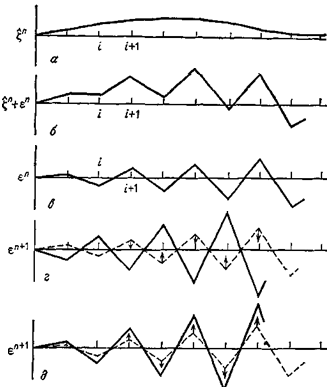
\includegraphics{{img/05/3.6}.png}
    \caption{Зростання похибки при використанні \eqref{eq:3.48}. а --- стаціонарний розв'язок на $n$-му шарі за часом; б --- збурений розв'язок на $n$-му шарі; в --- збурення на $n$-му шарі; г --- коливальне зростання похибки, пов'язане з надмірно великим кроком $\Delta t$ (динамічна нестійкість); д --- монотонне зростання похибки, обумовлене застосуванням центральних різниць для конвективного члена (статична нестійкість)}
    \label{fig:3.6}
\end{figure}

Після цього рівняння \eqref{eq:3.48} запишеться так:
\begin{equation}
    \label{eq:3.50}
    \frac{\zeta_i^{n + 1} - \zeta_i^n}{\Delta t} = - \frac{u \hat{\zeta}_{i + 1}^n - u \hat{\zeta}_{i - 1}^n}{2 \Delta x} + \alpha \frac{\hat{\zeta}_{i + 1}^n - 2 \hat{\zeta}_i^n + \hat{\zeta}_{i - 1}^n}{\Delta x^2} - \frac{u \epsilon_{i + 1}^n - u \epsilon_{i - 1}^n}{2 \Delta x} + \alpha \frac{\epsilon_{i + 1}^n - 2 \epsilon_i^n + \epsilon_{i - 1}^n}{\Delta x^2}.
\end{equation}

Сума перших двох членів у правій частині рівняння \eqref{eq:3.50} являє собою скінченно-різницеве значення $(\partial \hat{\zeta} / \partial t)_i^n$, рівне нулю в силу припущення, що на $n$-му часовому шарі існує стаціонарний розв'язок. Тоді рівняння \eqref{eq:3.50} зводиться до наступного:
\begin{equation}
    \label{eq:3.51}
    \zeta_i^{n + 1} - \zeta_i^n \equiv \Delta \zeta_i = \Delta t \frac{u \epsilon_{i + 1}^n - u \epsilon_{i - 1}^n}{2 \Delta x} + \alpha \Delta t \frac{\epsilon_{i + 1}^n - 2 \epsilon_i^n + \epsilon_{i - 1}^n}{\Delta x^2}.
\end{equation}

Перший член у правій частині рівняння \eqref{eq:3.51} дає зміну $\zeta$, обумовлену конвекцією, а другий --- обумовлену дифузією.
Розглянемо рівняння \eqref{eq:3.51} тільки з одним дифузійним членом і оцінимо його в точці $i$. Оскільки $\epsilon_{i + 1} > 0$, $\epsilon_i < 0$ і $\epsilon_{i - 1} > 0$, маємо
\begin{equation}
    \label{eq:3.52}
    \Delta \zeta_i = \alpha \Delta t \frac{\epsilon_{i + 1}^n - 2 \epsilon_i^n + \epsilon_{i - 1}^n}{\Delta x^2} > 0.
\end{equation}

Виходить, для всіх $\Delta t > 0$ приріст $\Delta \zeta_i$ додатній й прагне компенсувати від'ємне збурення $\epsilon_i$.
Аналогічно, розглядаючи $\Delta \zeta$ в точці $i + 1$, маємо $\epsilon_{i + 2} < 0$, $\epsilon_i < 0$ і $\epsilon_{i + 1} > 0$, тому
\begin{equation}
    \label{eq:3.53}
    \Delta \zeta_{i + 1} = \alpha \Delta t \frac{\epsilon_{i + 2}^n - 2 \epsilon_{i + 1}^n + \epsilon_i^n}{\Delta x^2} < 0.
\end{equation}
тобто додатнє збурення $\epsilon_{i + 1}$ коректується від'ємним приростом $\Delta \zeta_{i + 1}$. \medskip

Помітимо, що приріст $\Delta \zeta_i = \zeta_i^{n + 1} - \zeta_i^n$ (а також $\Delta \zeta_{i + 1}$ і т.д.) пропорційний кроку $\Delta t$. Якщо крок $\Delta t$ занадто великий, то поправка за рахунок збільшення $\Delta \zeta_i$  виявиться надмірною. Для таких занадто великих $\Delta t$ величина нового $\zeta_i^{n + 1}$ буде більше початкового збурення, як це показане на мал.~\ref{fig:3.6}(г):
\begin{equation}
    \label{eq:3.54}
    |\zeta_i^{n + 1}| > |\epsilon_i|
\end{equation}
і аналогічно
\begin{equation}
    \label{eq:3.55}
    |\zeta_{i \pm 1}^{n + 1}| > |\epsilon_{i \pm 1}|.
\end{equation}

Поява таких осциляцій наростаючої амплітуди, обумовлених надмірно великим кроком за часом, називається динамічною нестійкістю, яку можна усунути зменшенням кроку за часом, зробивши його менше деякого ``критичного кроку за часом'' $\Delta t_{\text{кр}}$. \medskip

Розглянемо тепер рівняння \eqref{eq:3.51} тільки з одним конвективним членом. Оцінимо це рівняння в точці $i$, вважаючи $u > 0$. Припустимо, що збурення коливається по $i$, а його амплітуда зростає з ростом $i$. Тому $u \epsilon_{i + 1} > 0$, $u \epsilon_{i - 1} > 0$, $u \epsilon_i < 0$ і 
\begin{equation}
    \label{eq:3.56}
    \Delta \zeta_i = - \Delta t \frac{u \epsilon_{i + 1}^n - u \epsilon_i^n}{2 \Delta x} < 0,
\end{equation}
тобто приріст $\zeta_i$, обумовлений конвекцією, від'ємний навіть при $\epsilon_i < 0$. Це означає, що похибка зростає монотонно (див. мал.~\ref{fig:3.6}(д)). Поява такої наростаючої похибки називається статичною нестійкістю, яку не можна усунути зменшенням кроку за часом і можна усунути тільки переходом до якої-небудь іншої скінченно-різницевої схеми. \medskip

Якщо просторовий напрямок зростання $\epsilon$ по відношенню до $u$ відрізняється від показаного на мал.~\ref{fig:3.6}, тобто якщо або $u < 0$, або амплітуда $\epsilon$ зменшується за $i$, то конвективний член стає статично стійким, але при достатньо великих $\Delta t$ ще може мати місце динамічна нестійкість. У будь-якій реальній задачі початкові похибки розподілені більш-менш випадково, і можна бути впевненим, що в деякий момент часу й у деякій точці їх розподіл буде схожий на зображений на мал.~\ref{fig:3.6} ``катастрофічний'' розподіл. \medskip

Якщо в рівняння \eqref{eq:3.51} входять і конвективний, і дифузійний члени, то вони взаємодіють. Як ми далі побачимо, для розглянутої різницевої схеми виникає обмеження на $\Delta t$, обумовлене дифузійним членом, і інше обмеження на $\Delta t$, що залежить від порівняльної величини статично нестійкого конвективного члена й статично стійкого дифузійного члена, тобто від числа Рейнольдса. 

\subsection{Дослідження стійкості}

Після того як був даний загальний опис стійкості, розглянемо методи дослідження стійкості, їх взаємозв'язки й їх порівняня. Ці методи будуть продемонстровані на прикладі різницевої схеми з різницями вперед за часом і центральними різницями по просторовій змінній у застосуванні до лінійного модельного рівняння \eqref{eq:3.18}.

\subsubsection{Метод дискретних збурень}

Метод дослідження стійкості, який ми називаємо методом дискретних збурень, являє собою узагальнення методу, уперше використаного Томом і Апельтом [1961] і розвиненого Томаном і Шевчиком [1966]. Цей метод повністю відповідає вже даному нами опису нестійкості. Він прямий і простий по ідеї, і може застосовуватися для аналізу як стійкості, так і властивості транспортивності, яке буде визначено далі. Ідея: у рівняння в деякій точці вводиться дискретне збурення величини   й прослідковується вплив цього збурення; скінченно-різницева схема буде стійкою, якщо збурення загасають.
Для простоти спочатку розглянемо рівняння (3.18) тільки з дифузійним членом і припустимо, що знайдений стаціонарний розв'язок   для всіх  . Введемо в розв'язок збурення   й з (3.18) за схемою з різницями вперед за часом і центральними різницями по просторовій змінній одержимо
  	(3.57)
або
 ,	(3.58)
 ,	(3.59)
де дифузійне число   визначається рівністю
  .	(3.60)
В силу вимоги стійкості ці збурення повинні загасати. Для першого кроку за часом це приводить до умови
 , 	(3.61)
або
 . 	(3.62)
Права нерівність є результатом вимоги статичної стійкості й автоматично виконується при додатних  , тобто при   й  . Ліва нерівність є вимогою динамічної стійкості й виконується при  . Якщо, слідуючи Томану й Шевчику [1966], вимагати, щоб чисельний розв'язок моделював фізичне явище, не допускаючи осциляцій, обумовлених надмірно великим кроком за часом, тобто щоб
 ,	(3.63)
то випливає обмеження
 . 	(3.64)
Нерівність (3.63), однак, не є умовою стійкості в розумінні зменшення амплітуди збурення. Якщо розглядати досить велику кількість шарів за часом, то буде потрібно виконання нерівності (3.64). Спочатку за схемою з різницями вперед за часом і центральними різницями по просторовій змінній (рівняння (3.18)) обчислимо збурення в сусідніх точках:
  .	(3.65)
Для наступного шару за часом одержимо
            	(3.66)
Знову будемо вимагати, щоб мало місце нерівність
 ,	(3.67)
звідки випливає
 .	(3.68)
Ліва нерівність виконується завжди, у той час як права накладає обмеження  .
Таким чином, розгляд першого часового шару приводить до умови , а другого — до умови  . Можна розглядати й наступні часові шари, які приводять до ще більш жорстких умов для  . Початкове одиничне збурення   в точці   асимптотично прямує до осцилюючого розподілу , де  — деяке збурення меншої амплітуди, як показано на мал. 3.7.
 
Рис. 3.7. Асимптотическое поширення одиничного збурення в у точці i для рівняння дифузії, що розв'язується за схемою з різницями вперед за часом і із центральними різницями по просторовим змінним, а — початкове збурення; б — збурення після одного кроку за часом, d = 3/4;  в — збурення після дуже великої кількості кроків за часом.

Таким чином, видно, що найбільш жорстка умова для   з'являється при такому типі розподілу збурень; починаючи розрахунки з таким осцилюючим збуренням  , накладеним на , і застосовуючи схему (3.18) з різницями вперед за часом і центральними різницями по просторовій змінної, одержуємо
 .	(3.69)
Вимога стійкості
 	(3.70)
дає
 ,	(3.71)
або
 . 	(3.72)

Для наступних часових шарів умова (3.72) не міняється. Таким чином, це умова для великих значень часу еквівалентно умові (3.64) — умові відсутності осциляцій, обумовлених надмірно великим кроком за часом, у випадку ізольованого збурення.
З формули (3.60) випливає, що при фіксованому кроці просторової сітки й фіксованому   умову   накладає обмеження на крок за часом:
 . 	(3.73)
Відзначимо, що обмеження, що накладається умовою (3.73), є важким у розумінні витрати часу для чисельного розв'язку рівняння дифузії. Припустимо, що розрахунки ведуться з деяким просторовим кроком   до деякого безрозмірного часу  , де    — максимально можливий крок за часом. Якщо треба повторити розрахунки із удвічі меншим просторовим кроком   (наприклад, для того, щоб проконтролювати зменшення похибок апроксимації), то треба брати крок за часом  . Виходить, щоб досягти того ж значення безрозмірного часу  , буде потрібно вчетверо більше кроків за часом, тобто   й  . Крім того, для розрахунків кожного часового шару буде потрібно вдвічі більше часу, тому що , а це означає, що число розрахункових точок у досліджуваній області зросло вдвічі. Таким чином, для одномірного випадку зменшення вдвічі кроку просторової сітки збільшує витрати машинного часу у 8 разів!
 У двовимірній задачі зменшення вдвічі кроків   і   збільшує число розрахункових точок у чотири рази, збільшуючи тим самим необхідний машинний час в 16 раз. У тривимірній задачі дифузії зменшення всіх трьох просторових кроків удвічі збільшує машинний час в 32 рази. У загальному випадку зменшення розміру кроку з   до   при розв'язку D-мірної задачі дифузії з використанням явної схеми з різницями вперед за часом і центральними різницями по просторових змінних збільшує машинний час у   разів. Ясно, що методи, у яких вдається уникнути умови стійкості (3.73), були б досить бажані.
В наведених вище міркуваннях припущення про стаціонарність розв'язку несуттєво. Якщо з збуреного рівняння відняти повне незбурене нестаціонарне рівняння, то вийде рівняння для зміни похибки
  	(3.74)
 з умовою стійкості   і т.д. Результати в цьому випадку будуть ті ж, що й вище.
Розглянемо тепер рівняння (3.18) з конвективним й дифузійним членами й без обмеження загальності покладемо  . (Якщо , то зміниться роль індексів   і  ). Знову застосуємо схему з різницями вперед за часом і центральними різницями по просторовій змінній, накладаючи на   в точці   збурення , що дасть
  	(3.75)
Дослідження цього рівняння не дає додаткової інформації в порівнянні з попереднім аналізом рівняння з одним тільки дифузійним членом, тому що на конвективних членах у точках   не позначається збурення в точці  . Застосовуючи схему з різницями вперед за часом і центральними різницями по просторовій змінній і в точці , одержуємо
  	(3.76)
або
 , 	(3.77)
де   — число Куранта, a , як і раніше. Для стійкості знову будемо вимагати, щоб
  	(3.78)
або
 . 	(3.79)
Ліва нерівність автоматично виконується при  . Права нерівність (вимога статичної стійкості) дає іншу необхідну умову стійкості:
 , 
або
  .	(3.80)
Звернувшись тепер до точки  , одержимо
  	(3.81)
і вимога стійкості   тут дає
 . 	(3.82)

Розглядаючи спочатку праву нерівність (3.82) (статична стійкість), одержуємо
 . 	(3.83)

Якщо член у квадратних дужках від'ємний, то ця нерівність буде справедливо для всіх  , якщо ж цей член додатній, то одержуємо
 . 	(3.84)

Оскільки знаменник додатній, умова (3.84) менш жорстка, ніж (3.80), і тому перекривається нею.
Дослідження лівої нерівності (3.82) (динамічна стійкість) дає
 . 	(3.85)
Якщо член у квадратних дужках додатній, то ця нерівність виконується для всіх  , якщо ж цей член від'ємний, то одержуємо
 ,	(3.86)
де знаменник додатній. Умова (3.86) також менш жорстка, ніж (3.80), і тому нею перекривається.
Таким чином, з аналізу стійкості рівняння, що включає конвективний і дифузійний члени, за допомогою методу дискретних збурень випливають дві необхідні умови — рівняння (3.73) і (3.80). Якщо поширити цей аналіз на наступні шари за часом, то можуть з'явитися інші більш обмежувальні умови, але метод аналізу при цьому стає дуже незручним. Помітимо (і це буде показано нижче), що аналіз стійкості по фон Нейману дає іншу умова (нерівність  ).
Крім того, якщо додержуватися роботи Томана й Шевчика [1966] і додатково вимагати відсутності в точці   осциляцій, обумовлених надмірно великим  кроком за часом, те повинне бути
 , 	(3.87)
а рівняння (3.81) дасть
 , 	(3.88)
тобто
  	(3.89)
або
 . 	(3.90)
У рівнянні переносу вихору   й член   являє собою сіткове число Рейнольдса   . Таким чином,   є число Рейнольдса, отримане по локальній швидкості й характерній довжині, рівній розміру кроку просторової сітки  . Для відсутності осциляцій, обумовлених надмірно великим кроком за часом, потрібно, щоб
 	(3.91)
незалежно від  . Якщо вимогу відсутності осциляцій (3.90) скомбінувати з умовою (3.73), що накладається дифузією, то в результаті виходять наступні обмеження: число Куранта   й  . Як побачимо надалі, ці обмеження є правильними.

\subsection{Завдання для самостійної роботи}

\shortHomeworkDescription{Використовуючи метод дискретних збурень, дослідити стійкість схеми з різницями проти потоку
\begin{equation}
    \label{eq:3.92}
    \frac{\zeta_i^{n + 1} - \zeta_i^n}{\Delta t} = - \frac{u \zeta_i^n - u \zeta_{i - 1}^n}{\Delta z}, \quad u > 0
\end{equation}
що відповідає модельному рівнянню руху нев'язкої рідини. Показати, що умова стійкості накладає на число Куранта обмеження $C = u \Delta t / \Delta x \le 1$ й що вона включає критерій відсутності осциляцій, обумовлених надмірно великим кроком за часом.}
